\usetikzlibrary{arrows.meta,calc}
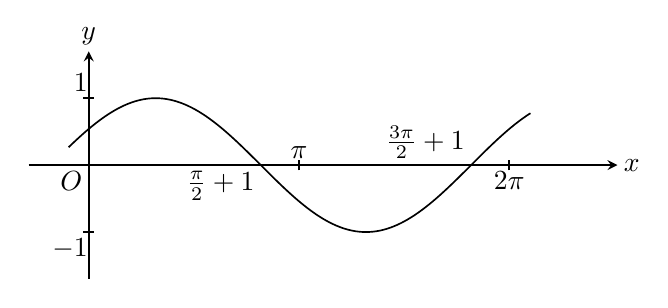
\begin{tikzpicture}[x=0.85cm,y=0.85cm,line width=.6pt,>=stealth]
\draw[->] (-0.9,0)--(7.9,0) node[right,inner sep=0pt,xshift=2pt] {$x$};
\draw[->] (0,-1.7)--(0,1.7) node[above,inner sep=0pt,yshift=2pt] {$y$};
\draw[domain=-0.3:6.6,samples=250] plot (\x,{cos(deg(\x-1))});
\draw (3.1415927,-0.08)--(3.1415927,0.08);
\draw (6.2831853,-0.08)--(6.2831853,0.08);
\draw (-0.08,1)--(0.08,1);
\draw (-0.08,-1)--(0.08,-1);
\node[anchor=north east,inner sep=0pt,xshift=-2pt,yshift=-2pt] at (0,0) {$O$};
\node[above left,inner sep=0pt,xshift=-2pt,yshift=2pt] at (0.08,1) {$1$};
\node[below left,inner sep=0pt,xshift=-2pt,yshift=-2pt] at (0.08,-1) {$-1$};
\node[below left,inner sep=0pt,xshift=-2pt,yshift=-2pt] at (2.5707963,0) {$\frac{\pi}{2}+1$};
\node[above,inner sep=0pt,xshift=0pt,yshift=2pt] at (3.1415927,0) {$\pi$};
\node[above left,inner sep=0pt,xshift=-2pt,yshift=2pt] at (5.712389,0) {$\frac{3\pi}{2}+1$};
\node[below,inner sep=0pt,xshift=0pt,yshift=-2pt] at (6.2831853,0) {$2\pi$};
\end{tikzpicture}
